\documentclass[a0paper,fleqn]{betterportraitposter}

% PACKAGES
\usepackage[none]{hyphenat}
\usepackage{lipsum}
\usepackage{qrcode} % QR code generation


\usepackage[utf8]{inputenc} % allow utf-8 input
\usepackage[T1]{fontenc}    % use 8-bit T1 fonts
\usepackage{url}            % simple URL typesetting
\usepackage{booktabs}       % professional-quality tables
\usepackage{amsfonts}       % blackboard math symbols
\usepackage{nicefrac}       % compact symbols for 1/2, etc.
\usepackage{microtype}      % microtypography
\usepackage{xcolor}         % colors

\usepackage{enumitem}

\usepackage{color}
\usepackage{float}
\usepackage[style=base]{caption}
\usepackage{subcaption}
\usepackage{tikz}
\usepackage{tikz-cd}
\usepackage{pgfplots}
\usepgfplotslibrary{groupplots}
\pgfplotsset{compat=1.18}

\usepackage{amsmath,amssymb,amsthm,mathtools,bbm}
\usepackage{physics}
\usepackage{bbold}
\usepackage{dsfont}
\usepackage{mathrsfs}
\usepackage[ruled,vlined,linesnumbered]{algorithm2e}
\usepackage[capitalize]{cleveref}
\usepackage{xfrac}
\usepackage{graphicx}
\usepackage{authblk}

\theoremstyle{plain}
\newtheorem{theorem}{Theorem}[section]
\newtheorem{proposition}[theorem]{Proposition}
\newtheorem{lemma}[theorem]{Lemma}
\newtheorem{corollary}[theorem]{Corollary}
\theoremstyle{definition}
\newtheorem{definition}[theorem]{Definition}
\newtheorem{assumption}[theorem]{Assumption}
\theoremstyle{remark}
\newtheorem{remark}[theorem]{Remark}

%%%% Uncomment the following commands to customise the format

%% Setting the height of the top and bottom (colored) bars
%% Uncomment either of the following lines it you want to change the defaults heights of the top or bottom bars.
\setlength{\mainfindingheight}{0.12\paperheight} % Top bar
\setlength{\centerboxheight}{0.77\paperheight} % Central box
\setlength{\bottomboxheight}{0.1\paperheight} % Bottom bar

%% Setting the page margin

%% Changing font sizes
% Text font
\renewcommand{\fontsizestandard}{\fontsize{28}{35} \selectfont}
% Main column font
\renewcommand{\fontsizemain}{\fontsize{100}{100} \selectfont}
% Title font
%\renewcommand{\fontsizetitle}{\fontsize{28}{35} \selectfont}
% Author font
%\renewcommand{\fontsizeauthor}{\fontsize{28}{35} \selectfont}
% Institution font
%\renewcommand{\fontsizeauthor}{\fontsize{28}{35} \selectfont}
% Section font
%\renewcommand{\fontsizesection}{\fontsize{28}{35} \selectfont}

%% Changing font sizes for a specific text segment
% Place the text inside brackets:
% {\fontsize{28}{35} \selectfont Your text goes here}

%% Changing colours
% Background of main claim box (options include: imperialblue, empirical, theory, methods and intervention
% Default is empirical
\renewcommand{\maincolumnbackgroundcolor}{imperialblue}

% Font on main and bottom boxes
% \renewcommand{\maincolumnfontcolor}{empirical}

% You can add a custom RGB color like so (example here is University of Glagow blue):
% \definecolor{UoGBurgundy}{RGB}{125, 35, 57}
% \renewcommand{\maincolumnbackgroundcolor}{UoGBurgundy}

\DeclareMathOperator*{\argmax}{arg\,max}
\DeclareMathOperator*{\erfc}{erfc}
\DeclareMathOperator*{\argmin}{arg\,min}

% partitin function
\newcommand{\Zbeta}{\ensuremath{\mathcal{Z}_\beta}}

\newcommand{\sign}{\ensuremath{\operatorname{sign}}}

% attack metrics
\newcommand{\advtrainingcost}{\ensuremath{\varepsilon_t}}
\newcommand{\advgencost}{\ensuremath{\varepsilon_g}}

% error metrics
\newcommand{\generr}{\ensuremath{E_{\mathrm{gen}}}}
\newcommand{\bounderr}{\ensuremath{E_{\mathrm{bnd}}}}
\newcommand{\trainerr}{\ensuremath{E_{\mathrm{train}}}}
\newcommand{\trainloss}{\ensuremath{\ell_{\mathrm{train}}}}
\newcommand{\advgenerr}{\ensuremath{E_{\mathrm{adv}}}}
\newcommand{\classpresgenerr}{\ensuremath{E_{\mathrm{CP}}}}
\newcommand{\usefulmetric}{\ensuremath{\mathcal{U}}}
\newcommand{\robustmetric}{\ensuremath{\mathcal{R}}}

% ERM definitions
\newcommand{\OptAttack}{\ensuremath{ \frac{\varepsilon_t \w^\top \Sigmadelta \w}{\sqrt{d} \sqrt{\w^\top \w}}}}
\newcommand{\RawPrediction}{\ensuremath{\frac{\boldsymbol{x}_\mu^\top \w }{\sqrt{d}}}}

% Covariances definitons
\newcommand{\Sigmaw}{\ensuremath{\boldsymbol{\Sigma}_{\boldsymbol{w}}}}
\newcommand{\Sigmax}{\ensuremath{\boldsymbol{\Sigma}_{\boldsymbol{\boldsymbol{x}}}}}
\newcommand{\Sigmadelta}{\ensuremath{\boldsymbol{\Sigma}_{\boldsymbol{\delta}}}}
\newcommand{\Sigmaupsilon}{\ensuremath{\boldsymbol{\Sigma}_{\boldsymbol{\upsilon}}}}
% \newcommand{\Sigmadeltainv}{\ensuremath{\boldsymbol{\Sigma}_{\boldsymbol{\delta}}^{-1}}}
\newcommand{\Sigmatheta}{\ensuremath{\boldsymbol{\Sigma}_{\boldsymbol{\theta}}}}

% w's definitions
\newcommand{\w}{\ensuremath{\boldsymbol{\theta}}}
\newcommand{\x}{\ensuremath{\boldsymbol{x}}}
\newcommand{\wavec}{\ensuremath{\boldsymbol{\theta}^a}}
% \newcommand{\wstar}{\ensuremath{\boldsymbol{w}^\star}}
\newcommand{\what}{\ensuremath{\hat{\boldsymbol{\theta}}}}
\newcommand{\wstar}{\ensuremath{\boldsymbol{\theta}_0}}
\newcommand{\vecdelta}{\ensuremath{\boldsymbol{\delta}}}
\newcommand{\singleattack}{\ensuremath{\boldsymbol{v}}}

% indices
\newcommand{\datidx}{\ensuremath{i}}
\newcommand{\blockidx}{\ensuremath{\ell}}


% proximal and moreau
\newcommand{\proxim}[3]{\ensuremath{\mathcal{P}_{#1}\qty[#2]\qty(#3)}}
\newcommand{\Dproxim}[3]{\ensuremath{\mathcal{P}^\prime_{#1}\qty[#2]\qty(#3)}}
\newcommand{\moreau}[3]{\ensuremath{\mathcal{M}_{#1}\qty[#2]\qty(#3)}}
\newcommand{\Dmoreau}[3]{\ensuremath{\mathcal{M}^\prime_{#1}\qty[#2]\qty(#3)}}


\newcommand{\gaussdist}[2]{\ensuremath{\mathcal{N}\qty(#1, #2)}}

\newcommand{\outputfun}{\ensuremath{f_{\mathrm{out}}}}
\newcommand{\priorfun}{\ensuremath{f_{\mathrm{w}}}}

\newcommand{\pout}[1]{\ensuremath{P_{\mathrm{out}}\qty(#1)}}
\newcommand{\poutbayes}[1]{\ensuremath{P_{\mathrm{out}^\star}\qty(#1)}}
\newcommand{\Zout}{\ensuremath{\mathcal{Z}_{\mathrm{out}}}}
\newcommand{\Zoutstar}{\ensuremath{\mathcal{Z}_{\mathrm{out}^\star}}}
\newcommand{\Zw}{\ensuremath{\mathcal{Z}_{\mathrm{w}}}}
\newcommand{\Zwstar}{\ensuremath{\mathcal{Z}_{\mathrm{w}^\star}}}
\newcommand{\fout}{\ensuremath{f_{\mathrm{out}}}}
\newcommand{\foutstar}{\ensuremath{f_{\mathrm{out}^\star}}}
\newcommand{\fw}{\ensuremath{f_{\mathrm{w}}}}
\newcommand{\fwstar}{\ensuremath{f_{\mathrm{w}^\star}}}

 
\newcommand{\PP}[1]{\ensuremath{\mathbb{P}\qty(#1)}}
\newcommand{\EE}[1]{\ensuremath{\mathbb{E}\qty[#1]}}
\newcommand{\EEb}[2]{\ensuremath{\mathbb{E}_{#1}\qty[#2]}}
\newcommand{\RR}{\ensuremath{\mathbb{R}}}

\newcommand{\din}{\ensuremath{\Delta_{\text{\tiny{IN}}}}}
\newcommand{\dout}{\ensuremath{\Delta_{\text{\tiny{OUT}}}}}
\newcommand{\deff}{\ensuremath{\Delta_{\text{eff}}}}

\newcommand{\zetain}{\ensuremath{\zeta_{\text{\tiny{IN}}}}}
\newcommand{\zetaout}{\ensuremath{\zeta_{\text{\tiny{OUT}}}}}

\newcommand{\chiin}{\ensuremath{\chi_{\text{\tiny{IN}}}}}
\newcommand{\chiout}{\ensuremath{\chi_{\text{\tiny{OUT}}}}}

\newcommand{\lambdaout}{\ensuremath{\lambda_{\text{\tiny{OUT}}}}}
\newcommand{\lambdaopt}{\ensuremath{\lambda_{\mathrm{opt}}}}

\newcommand{\zetainzero}{\ensuremath{\zeta_{\text{\tiny{IN}},0}}}
\newcommand{\zetaoutzero}{\ensuremath{\zeta_{\text{\tiny{OUT}},0}}}

\newcommand{\ginzero}{\ensuremath{g_{\text{\tiny{IN}},0}}}
\newcommand{\goutzero}{\ensuremath{g_{\text{\tiny{OUT}},0}}}

\newcommand{\yin}{\ensuremath{y_{\text{\tiny{IN}}}}}
\newcommand{\yout}{\ensuremath{y_{\text{\tiny{OUT}}}}}
\newcommand{\ystar}{\ensuremath{y^\star}}

\newcommand{\losshuber}[1]{{\ell^{\rm Huber}_{#1}}}


\newcommand{\aopt}{\ensuremath{a_{\text{\tiny{opt}}}}}
\newcommand{\aoptzero}{\ensuremath{a_{\text{\tiny{opt}},0}}}



\newcommand{\isEquivTo}[1]{\ensuremath{\underset{#1}{\simeq}}}

\newcommand{\Egen}{\ensuremath{E_{\mathrm{gen}}}}
\newcommand{\Egenbest}{\ensuremath{E_{\mathrm{gen}}^{\mathrm{best}}}}
\newcommand{\Eest}{\ensuremath{E_{\mathrm{estim}}}}
\newcommand{\excessEgen}{\ensuremath{E_{\mathrm{gen}}^{\mathrm{excess}}}}
\newcommand{\Etrain}{\ensuremath{E_{\mathrm{train}}}}

\newcommand{\ntest}{\ensuremath{n_{\mathrm{t}}}}

\newcommand{\qb}{\ensuremath{q_{\mathrm{b}}}}


\begin{document}	

%% Top box with main message
\mainfinding{

    A \textbf{rigorous, closed-form characterisation} of
    \textbf{adversarial generalisation errors}.

    % A High Dimensional Statistical Model for \textbf{Adversarial Training}: Geometry and Trade-Offs

    % \textbf{Adversarial training} protects the \textbf{non-robust} features. 
    % \newline
    % A \textbf{trade-off} emerges if those features are \textbf{useful}.

}


% Title, author and affiliations section
\titlebox{
    \title{A High Dimensional Statistical Model for Adversarial Training: Geometry and Trade-Offs}  
    }
% End of title stuff
    
%% Central box with traditional content
\centerbox{
\begin{multicols}{3}

\section{Binary Classification}

\textbf{Teacher-Student Setting}: Training data \(\mathcal{D} = \qty{(\x_\datidx, y_\datidx)}_{\datidx=1}^{n}\in\mathbb{R}^{d}\times\{-1,+1\}\) where \(\x_\datidx \sim \gaussdist{\boldsymbol{0}}{\Sigmax}\) and \(y_{i} \sim \mathbb{P}(y|\wstar^{\top}\x_{i})\)
for fixed $\wstar\in\mathbb{R}^{d}$.

Focus on probit model \(\mathbb{P}\left(y|z\right) = \sfrac{1}{2}\erfc\left(-\sfrac{z}{\sqrt{2}\tau}\right)\), with noise parameter $\tau > 0$.

\textbf{Problem Statement}: Learn \(\hat{y}(\what(\mathcal{D}), \x) = \sign ( \what(\mathcal{D}) \cdot \x / \sqrt{d})\) using adversarial training.

\textbf{Generalisation Error}: 
\begin{equation}\label{eq:gen-error-definition}
    \generr = \EEb{y,\x}{
        \mathbb{1}(y \neq \hat{y} (\what, \x))
    } \,,
\end{equation}

\textbf{Adversarial Attack}: 
Chose \(\norm{\boldsymbol{\upsilon}}_{\Sigmaupsilon^{-1}} \leq \advgencost\) to misclassify the sample \(\x_\datidx\): \(y(\x_\datidx) \neq \hat{y}(\what, \x_\datidx + \boldsymbol{\upsilon}_\datidx)\).

\textbf{Adversarial Generalisation Error}: 
\begin{equation}\label{eq:adv_gen_metric_definition}
    \advgenerr = \EEb{y,\x}{
        \max_{\norm{\vecdelta}_{\Sigmaupsilon^{-1}} \leq \advgencost} \mathbb{1}(y \neq \hat{y} (\what, \x + \vecdelta))
    } \,, 
\end{equation}
Note, \(\generr = \advgenerr(\advgencost=0)\). 

\textbf{Boundary Error}: 
\(\advgenerr = \generr + \bounderr\) where \(\bounderr\) are the attackable samples.

\section{Adversarial ERM}

\begin{equation}\label{eq:adversarial-training-problem}
     \sum_{\datidx = 1}^{n} 
    \max_{
        \norm{\vecdelta_\datidx}_{\Sigmadelta^{-1}} \leq \advtrainingcost 
    }
    g \qty(y_\datidx \frac{\w^\top \qty(\x_\datidx + \vecdelta_\datidx)}{\sqrt{d}}) 
    + r(\w) \,,
\end{equation}
where \(g\) is a convex loss, \(r(\w)\) is a convex regularisation and \(\Sigmadelta\) is positive definite. 
We set \(r(\w) = \frac{\lambda}{2} \norm{\w}_2^2\).

The inner maximisation has a closed form solution:
\begin{equation}\label{eq:modified-minimisation-problem}
    \sum_{\datidx = 1}^{n} 
    g \qty(
        y_\datidx \frac{\w^\top \x_\datidx}{\sqrt{d}} 
        - \advtrainingcost \frac{\sqrt{\w^\top \Sigmadelta \w}}{\sqrt{d}} 
    ) 
    + r(\w) \,.
\end{equation}

\textbf{The High-Dimensional Proportional Limit (hdl)}. The dimension \(d\) and the number of training samples \(n\) are large \(d,n \to \infty\), but the sample complexity is fixed \(\alpha := n / d\).


\subsection{Usefulness and robustness}
Usefulness relates to generalisation error and robustness relates to boundary error.
\begin{align}
   \usefulmetric_{\wstar}
   &= \frac{1}{\sqrt{d}} \mathbb{E}_{\x, y}[y \wstar^\top \x ] \,, \label{eq:mt-usefulness-def} \\
   \robustmetric_{\wstar} &= \frac{1}{\sqrt{d}} \EEb{\x, y}{
       \inf_{\norm{\vecdelta}_{\Sigmaupsilon^{-1}}  \leq \advgencost} y \wstar^\top ( \x + \vecdelta)
   }\,. \label{eq:mt-robustness-def}
\end{align}

\subsection{Block Features}
Craft artificial usefulness and robustness:
\begin{equation}
\begin{aligned}
   \Sigmax &= \operatorname{blockdiag}\qty( \psi_1 \mathbb{1}_{d_1}, \dots, \psi_k \mathbb{1}_{d_k} ) \,, \\
   \Sigmadelta &= \operatorname{blockdiag}\qty( \Delta_1 \mathbb{1}_{d_1}, \dots, \Delta_k \mathbb{1}_{d_k} ) \,, \\
   \Sigmaupsilon &= \operatorname{blockdiag}\qty( \Upsilon_1 \mathbb{1}_{d_1},  \dots, \Upsilon_k \mathbb{1}_{d_k} ) \,, \\
   \Sigmatheta &= \operatorname{blockdiag}\qty( t_1 \mathbb{1}_{d_1}, \dots, t_k \mathbb{1}_{d_k} ) \,,
\end{aligned}
\end{equation}


\section{Main Theorem}
\textbf{Assumptions}: 
\begin{itemize}
    \item Well defined spectral distribution in the hdl \(\Sigmax = \mathrm{S}^\top \operatorname{diag}(\omega_i) \mathrm{S}\), \(\zeta_i = \operatorname{diag}(\mathrm{S} \Sigmadelta \mathrm{S}^\top)_{i}\) and \(\upsilon_i = \operatorname{diag}(\mathrm{S} \Sigmaupsilon \mathrm{S}^\top )_i\).
    \item Assume that \(\wstar^\top \Sigmax \wstar / d\) converges to \(\rho\) in the limit and that the entries of \(\bar{\boldsymbol{\theta}} = \mathrm{S} \Sigmax^\top \wstar / \sqrt{\rho}\) converge as well to a limiting distribution.
    \item Assume that in the hdl the spectral distributions for the matrices and the distributions of the elements of the vectors just defined converge jointly to a p.d.f., \textit{i.e.} \(\nicefrac{1}{d} \sum_{i=1}^{d} \delta(\omega - \omega_i)\delta(\bar{\theta} - \bar{\theta}_i) \delta(\zeta - \zeta_i)\delta(\upsilon - \upsilon_i) \to \mu(\omega, \bar{\theta}, \zeta, \upsilon)\).
\end{itemize}


For \(\lambda \geq 0\)
\begin{align}
    \generr &= \frac{1}{\pi} \arccos \qty( 
    {
        m / \sqrt{ (\rho + \tau^2) q}
    } 
    ) \,, \\
    % \advgenerr &= \generr +  
    \bounderr &= \!
    % \int_{0}^{\advgencost \frac{A}{\sqrt{q}\sqrt{N}}} 
    \int_{0}^{\advgencost \frac{\sqrt{A}}{\sqrt{q}}} \!\!\!\!
    {\textstyle
        \erfc\left( \frac{ -\frac{m}{\sqrt{q}} \nu}{\sqrt{2 \qty(\rho + \tau^2 - m^2 / q)}} \right) 
        \!\! \frac{e^{-\frac{\nu^2}{2}}}{\sqrt{2\pi}} \dd{\nu}
    }
    % \mathcal{D}_1 \qty[\nu] 
    \label{eq:adv-error-theorem-overlap} \,, 
\end{align}
and \(\advgenerr = \generr + \bounderr\).

\((m, q, V, P, \hat{m}, \hat{q}, \hat{V}, \hat{P})\) are the solutions of the following system of equations.
Four are dependent on the loss function \(g\) and the adversarial training strength \(\advtrainingcost\):
\begin{equation}\label{eq:saddle-point-channel-main-thm}§
    \begin{cases}
        \hat{m} = \alpha \mathbb{E}_{\xi}\left[
            \int_{\RR} \dd{y} \partial_\omega \mathcal{Z}_0 f_g(y, \sqrt{q} \xi, P)
        \right] \\
        \hat{q} = \alpha \mathbb{E}_{\xi}\left[
            \int_{\RR} \dd{y} \mathcal{Z}_0 f_g^2(y, \sqrt{q} \xi, P)
        \right] \\
        \hat{V} = -\alpha \mathbb{E}_{\xi}\left[
            \int_{\RR} \dd{y} \mathcal{Z}_0 \partial_\omega f_g(y, \sqrt{q} \xi, P)
        \right] \\
        \hat{P} = - \frac{\advtrainingcost}{2 \sqrt{P}} \alpha \mathbb{E}_{\xi} \qty[ 
            \int_{\RR} \dd{y} y \mathcal{Z}_0 f_g (y, \sqrt{q} \xi, P)
        ] 
    \end{cases} \,,
\end{equation}
where \(\xi \sim \gaussdist{0}{1}\) and 
\(\mathcal{Z}_{0} = \nicefrac{1}{2} \erfc(\nicefrac{- y \omega}{ \sqrt{2(V + \tau^2)}})\) and \(f_{g}(y, \omega, V, P) = \qty(\mathcal{P}(\omega) - \omega) / V\), where \(\mathcal{P}\) is the following proximal operator
\begin{equation}
    \mathcal{P} (\omega) = \min_x \qty[\frac{(x - \omega)^2}{2 V} + g(yx - \advtrainingcost \sqrt{P})] \,.
\end{equation}
The other four are dependent on the spectral distribution of the matrices \(\Sigmax, \Sigmadelta\) and on the limiting distribution of the elements of \(\bar{\boldsymbol{\theta}}\):
\begin{equation}\label{eq:saddle-point-prior-main-thm}
    \begin{cases}
        m = \mathbb{E}_{\mu} \qty[ 
            \frac{\hat{m} \bar{\theta}^2}{\lambda + \hat{V} \omega + \hat{P} \delta} 
        ] \\
        q = \mathbb{E}_{\mu} \qty[ 
            \frac{
                \hat{m}^2 \bar{\theta}^2 \omega + \hat{q} \omega^2
            }{
                (\lambda + \hat{V} \omega + \hat{P} \delta)^2
            } 
        ] \\
        V = \mathbb{E}_{\mu} \qty[ 
            \frac{\omega}{\lambda + \hat{V} \omega + \hat{P} \delta } 
        ] \\
        P = \mathbb{E}_{\mu} \qty[ 
            \zeta \frac{
                \hat{m}^2 \bar{\theta}^2 + \hat{q} \omega^2
            }{
                (\lambda + \hat{V} \omega + \hat{P} \delta)^2
            } 
        ] 
    \end{cases}\,.
\end{equation}
\(A\) is given by
\begin{equation}
    A = \! \mathbb{E}_{\mu} \! \qty[ 
    {\textstyle
        \upsilon \frac{\hat{m}^2 \bar{\theta}^2 \omega + \hat{q} \omega^2}{(\lambda + \hat{V} \omega + \hat{P} \delta)^2} 
    }
    ] \,.
\end{equation}
\(m,q,P\) and \(A\) are interpretable:
\begin{equation}\label{eq:interpretation-overlaps}
\begin{aligned}
    m &= {\textstyle \mathbb{E}_{\mathcal{D}}\qty[\frac{1}{d} \wstar^\top \Sigmax \what] }\,, & \  
    q &= {\textstyle \mathbb{E}_{\mathcal{D}}\qty[\frac{1}{d} \what^\top \Sigmax \what] }\,, \\
    P &= {\textstyle \mathbb{E}_{\mathcal{D}}\qty[\frac{1}{d} \what^\top \Sigmadelta \what] } \,, &\ 
    A &= {\textstyle \mathbb{E}_{\mathcal{D}}\qty[\frac{1}{d} \what^\top \Sigmaupsilon \what] } \,.
\end{aligned}
\end{equation}

\section{Trade-Offs}

\begin{equation}
    \advgenerr = 
    {
        \generr(\vartheta, \usefulmetric_{\wstar}) + 
        \int_{0}^{\advgencost \varkappa } 
        f(\xi; \vartheta, \usefulmetric_{\wstar}) \dd{\xi}
    } \,,
\end{equation}
where we introduce the variable \(\vartheta = m / \sqrt{\rho q}\) and \(\varkappa = \sqrt{A} / \sqrt{q}\). 
\(\vartheta\) is the cosine of the angle between the teacher weights \(\wstar\) and the student estimate \(\what\) in the geometry of \(\Sigmax\) and \(\varkappa\) is the norm of \(\what\) under the attack matrix.
The function \(f(\xi;\vartheta)\) is positive \(\forall \vartheta, \forall \xi \in [0, +\infty)\) and it is strictly increasing in \(\vartheta\) for any fixed \(\xi \in [0,+\infty)\). 

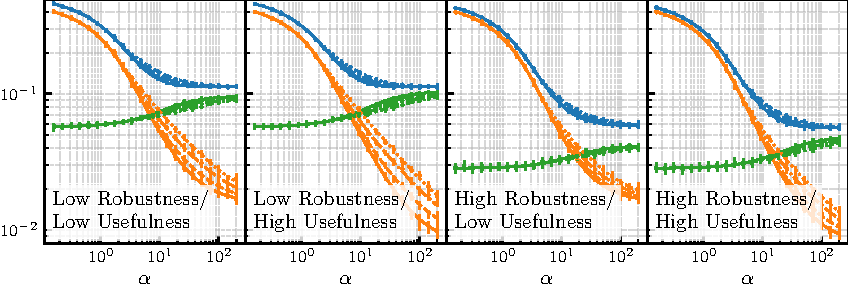
\includegraphics[width=0.2\textwidth]{Assets/feature_combinations_alpha_sweep.pdf}


We notice that the values for \(\generr\) and \(\bounderr\) change by varying the usefulness and robustness of the features for fixed types of attacks. 
Intuitively, we have that the more usefulness one has the less generalisation error one makes, indeed we can write a lower bound for the generalisation error
\begin{equation}\label{eq:bound-gen-error}
    \generr
    \geq
    \frac{1}{\pi} \arccos( \sqrt{\frac{\pi}{2 \rho}} \usefulmetric_{\wstar} ) \,. 
\end{equation}
We note that \(\rho\) and \(\usefulmetric_{\wstar}\) only depend on \(\Sigmax\) and \(\wstar\).

Robustness only affects the boundary error. 
High robustness implies less sensibility to adversarial attacks: robust features have less samples within an attack range of the student decision boundary. 
The highest value that the boundary error can achieve is limited by both the robustness and the usefulness as
\begin{align} \label{eq:bound-boundary-error}
    \bounderr \leq & \  
    2 \mathrm{T}\qty( \advgencost \mathcal{A} \, \mathcal{B}, \mathcal{A}^{-1} ) - \frac{1}{\pi} \arctan( \mathcal{A}^{-1} ) \nonumber\\ 
    & - \frac{1}{\pi} \erf\qty( \frac{\advgencost \mathcal{B}}{\sqrt{2}} ) \erfc\qty( \frac{\advgencost \mathcal{A} \, \mathcal{B}}{\sqrt{2}} ) \,,
\end{align}
where \(\mathcal{B} = \max_i \sqrt{(\Sigmaupsilon)_{ii} / (\Sigmax)_{ii}}\), \(\mathcal{A} = \sqrt{\pi} \usefulmetric_{\wstar} / \sqrt{2 \rho}\) and \(\mathrm{T}\) is the Owen function. This previous bound is a decreasing function of the robustness.


Under the same setting as \cref{thm:main-theorem-saddle-point-eqs} and considering a BFM with a single type of feature, i.e. \(k=1\) one has that \(\forall \advgencost, \advtrainingcost \geq 0\) for \(\alpha\) big enough 
exist two positive numbers $M_1, M_2$ such that
\begin{equation}
\begin{aligned}
    \abs{
        \advgenerr(\advgencost, \advtrainingcost) - \advgenerr(\advgencost,  \advtrainingcost = 0)
    } & < M_1 / \alpha \,, \\
    % \to 0 \,, \\
    \abs{
        \generr(\advtrainingcost) - \generr(\advtrainingcost = 0)
    } & < M_2 / \alpha \,,
    % \to 0 \,.
\end{aligned}
\end{equation}
where \(\advgenerr(\advgencost, \advtrainingcost)\) and \(\generr(\advtrainingcost)\) define the adversarial and generalisation error of \(\what\) trained with \(\advtrainingcost\) and evaluated for \(\advgencost\).

\subsection{Directional Defences and structured data}

Consider the SWFM defined in \cref{sec:strong-weak-feature-model}
where the defence matrix is 
\(
    \Sigmadelta = \operatorname{blockdiag}\qty( 
        (\Delta_1 + \delta_1 \varrho ) \mathbb{1}_{d_1}, (\Delta_2 + \delta_2 \varrho ) \mathbb{1}_{d_2} 
    )
\), 
with \(\varrho\) the parameter that makes the defence matrix change.
Assume also that \(\psi_1 > \psi_2\), \(\Delta_2 \psi_1 \geq \Delta_1 \psi_2\) and \(\Upsilon_i = 1\).
In the \(\alpha\to \infty\) (taken after the \(n,d\to\infty\)) there exists \(\kappa > 0\) such that \(\forall \delta_1 > \kappa\), \(\delta_2 = -\delta_1\) one has that
\begin{equation}
\begin{aligned}
    \bounderr(\varrho) &= \bounderr^0 + \bounderr^1 \varrho + \order{\varrho^2} \,, \\
    \generr(\varrho) &= \generr^0 + \generr^1 \varrho + \order{\varrho^2} \,,
\end{aligned}
\end{equation}
where \(\generr^1 > 0\), \(\bounderr^1 < 0\) and \(\bounderr^0,\generr^0\) are the errors when \(\varrho =0\).
Additionally, this leads to an improved value of \(\advgenerr\) at order \(\varrho\) iff the following condition is satisfied
\vspace{-5pt}
\begin{equation}
    {\textstyle
        \frac{\advgencost}{\sqrt{2}}
        \erfc\qty( -\frac{\vartheta_0 u_0 \advgencost}{ \sqrt{2-2 \vartheta_0 ^2} }) 
        < \frac{e^{-\frac{\vartheta_0^2 u_0^2 \advgencost ^2}{2 \left(1-\vartheta_0 ^2\right) } }}{\sqrt{\pi} \sqrt{1-\vartheta_0^2}} \,,
    }
\end{equation}
% \(
%     \sqrt{\pi} \sqrt{1-\vartheta_0^2} \advgencost  
%     \erfc\qty( -\vartheta_0 u_0 \advgencost / \sqrt{2-2 \vartheta_0 ^2} ) 
%     \leq 
%     \sqrt{2} \exp\qty(\vartheta_0^2 u_0^2 \advgencost ^2 / (2 \left(\vartheta_0 ^2-1\right) ) )
% \)
where \(\vartheta_0 = m_0 / \sqrt{\rho q_0}\) and \(u_0 = \sqrt{A_0} / \sqrt{q_0}\) the solution of the problem with \(\varrho = 0\). 
Notice that for \(\advgencost\) small enough this condition is always verified.

\begin{center}
    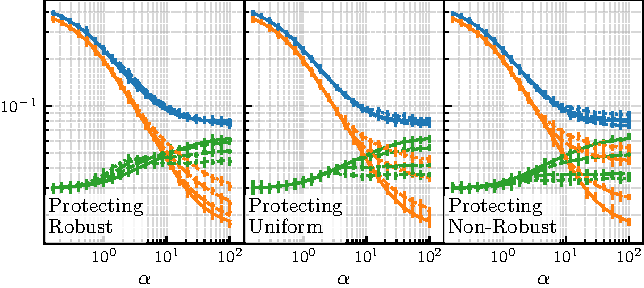
\includegraphics[width=0.2\textwidth]{Assets/defence_sweep.pdf}
    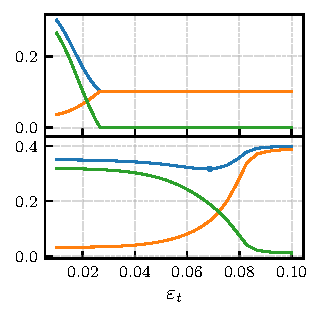
\includegraphics[width=0.1\textwidth]{Assets/optimal_defense.pdf}
    \postercaption{TODO add caption}
\end{center}



\subsection{Tradeoff directions and innocuous directions}
We now investigate the effect that different types of geometries have on the trade-off between \(\generr\) and \(\bounderr\). 
% One can ask what this the effect of the different eigenvectors of \(\Sigmaupsilon\) on the adversarial generalisation error. 
Depending on the attack geometry \(\Sigmaupsilon\) one can choose different defence geometries \(\Sigmadelta\) and ask if and for which, protection without trade-off is possible. 
% This question translates to asking if we can minimise \cref{eq:simplified-adv-error-formula} with respect to \(\varkappa = \sqrt{A} / \sqrt{q}\) and \(\vartheta = m / \sqrt{\rho q}\).
Any attack matrix \(\Sigmaupsilon\) eigenvalues can be split into 
directions orthogonal to the teacher and directions aligned with the teacher. 
% where both have very different roles in the adversarial trade-off. 
\Cref{fig:optimal_defense} (Left) considers the effect of the adversarial training strength \(\advtrainingcost\) on the errors for different choices of matrices \(\Sigmadelta = \Sigmaupsilon\). 
In the the top we consider matrices whose biggest eigenvalues are orthogonal to the teacher vector and in the bottom one matrices where there is a leading eigenvector in the direction of the teacher.




\subsection{Data Dependent Regularisation}

The form for the approximate loss in the case of small \(\advtrainingcost\) is
\begin{equation}\label{eq:equivalent-adversarial-regularisation}
    \sum_{\datidx = 1}^{n} 
    g \Big( y_\datidx \frac{\w^\top \x_\datidx}{\sqrt{d}} \Big) 
    + \tilde{\lambda}_1 \sqrt{\w^\top \Sigmadelta \w} + \tilde{\lambda}_2 \w^\top \Sigmadelta \w
\end{equation}
where \(\tilde{\lambda}_1\) and \(\tilde{\lambda}_2\) depend on the model's parameters and perturbed margins of the points that shift sign under perturbation. 

\begin{center}
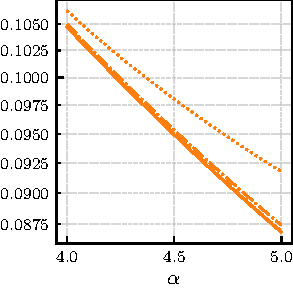
\includegraphics[width=0.15\textwidth]{Assets/gen_lambda_optimal_sweep_alpha.pdf}
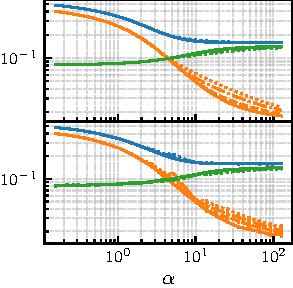
\includegraphics[width=0.15\textwidth]{Assets/effective_regularisation.pdf}
\postercaption{TODO better caption}
\end{center}

\section{Acknowledgements}

Bruno Loureiro acknowledges support from the \textit{Choose France - CNRS AI Rising Talents} program, and Florent Krzakala from the Swiss National Science Foundation grant SNFS OperaGOST  (grant number $200390$).





\columnbreak

\end{multicols}
}




% End of central box

% Bottom box with QR code
\bottombox{
    %% QR code
    \qrcodecommand{https://arxiv.org/abs/2402.05674}{

    Kasimir Tanner
    \newline
    Matteo Vilucchio
    \newline
    Bruno Loureiro
    \newline
    Florent Krzakala
    \newline

}
}{
    % Comment out the line below out to hide logo
    \hfill\bottomboxlogo{Assets/EPFL_Logo_Digital_RGB_PROD.png} % \hfill shifts the logo across so it meets the right hand side margin
    % Note that \bottomboxlogo takes an optional width argument. It defaults to the following: 
    % \hfill\bottomboxlogo[width=\textwidth]{<path_to_image_file>} 
    % where \textwidth is actually the width of a minipage which is defined in the \bottombox command of
    % betterportaitposter.cls It's a standard \includegraphics command in there, so easy to change if 
    % you need to add a border etc.
}
% End of bottom box



\end{document}